\documentclass[12pt]{article}
\usepackage[T1]{fontenc}
\usepackage{indentfirst}
\usepackage{anyfontsize}
\usepackage{setspace}
\usepackage{titlesec}
\usepackage[romanian]{babel}
\usepackage{graphicx}
\usepackage{quiver} 
%\usepackage{helvet}
%\renewcommand{\familydefault}{\sfdefault}

\usepackage{geometry}
 \geometry{
 a4paper,
 total={210mm,297mm},
 left=20mm,
 right=20mm,
 top=25mm,
 bottom=20mm,
 }
\setlength\parindent{15mm}

\begin{document}

\fontsize{20pt}{18pt}\selectfont
\title{\textbf{Microprocesorul RISC-V}}
\date{}
\maketitle

\vspace*{150mm}


\begingroup
    \fontsize{14pt}{12pt}\selectfont
	\textbf{Canditat: Dan-Alexandru Bulzan}
	\bigbreak
	\textbf{Coordonator științific: Ș.l.dr.ing Eugen-Horațiu Gurban}
\endgroup


\vspace*{\fill}
\begin{center}
\fontsize{14pt}{12pt}\selectfont
Sesiune: Iunie 2024
\end{center}


\newpage
\section{\centering INTRODUCERE}
\bigbreak
\subsection{SCOPUL ȘI MOTIVAȚIA LUCRĂRII}
\setstretch{1.2}

Implementarea personală a setului de instrucțiuni RISC-V, s-a născut din dorința de a realiza ceea ce poate fi considerat nimic mai puțin decât un apogeu al metodelor științifice din ultimul secol, și anume, procesorul.

Aceste dispozitive electronice reprezintă fundamentul tuturor științelor informatice, grație capacității computaționale intrinsece. Procesoarele, indiferent de gradul lor de specializare, au fost și rămân nucleul unei revoluții tehnologice pe care nici din pură ignoranță nu o putem omite, aceasta fiind prezentă până și în cele mai mundane aspecte ale vieții cotidiene.
Scopul acestei lucrări este de a traversa universul digital, începând din rădăcinile sale analogice, ajungând într-un final la organizarea ierarhică a numeroaselor entități digitale în a căror întregime se constituie un sistem de calcul complet funcțional.

Adesea este usor sa ne pierdem în complexitățiile ascunse printre miile de porți logice, un veritabil microcosm digital, însă prin mijloacele abstractizării și modularizării, proiectarea unui procesor devine nimic mai mult decât o modelare regulată a unui sistem descriptibil de operațiile algebrei Booleane. Pe parcursul lucrării, se va prezenta de asemenea o simplă implementare didactică a modulului de memorie cache, un component digital de o importanță deosebită, precum si problematica care cere o astfel de soluție.

Implementarea va fi realizată în limbajul de descriere hardware VHDL, entitățile urmând să fie simulate prin intermediul Vivado, soluție de design și sinteză hardware oferită de Advanced Micro Devices.

\begin{center}
\vspace*{40mm}
DE CONTINUAT, ALTERAT
\end{center}

\newpage
\section{\centering STUDIU BIBLIOGRAFIC}
\bigbreak
\subsection{ARHITECTURA RISC}
Înainte de realizarea unei analize asupra stadiului de dezvoltare și implementare al setului de instrucțiuni RISC-V, întelegerea locului pe care filozofia RISC o are în disciplina arhitecturii calculatoarelor, este de o importantă deosebită.

Acronimul RISC, face referintă la \textit{reduced instruction set computer} sau calculator cu set de instrucțiuni reduse. Un microprocesor care implementează o astfel de filozofie, utilizează un set de instructiuni compact și puternic optimizat, garantând execuția rapidă a fiecărei instrucțiuni. Prin urmare, o caracteristică a acestei abordări, este faptul că microprocesorul va fi nevoit să execute un numar mai ridicat de instrucțiuni pentru a realiza aceleași operații efectuate de un calculator cu set de instrucțiuni complex, cunoscut și sub acronimul de \textit{CISC}, printr-un număr observabil mai redus de instrucțiuni.

De-a lungul timpului, începând cu întemeierea arhitecturii RISC, au fost conceput mai multe seturi de instrucțiuni relevante, printre acestea enumerându-se următoarele: MIPS, ARM cât și setul care va reprezenta arhitectura procesorului implementat pe decursul acestei lucrari, RISC-V.

\subsection{FAMILIA SETURILOR DE INSTRUCȚIUNI ARM}
Seturile de instrucțiuni care aparțin familiei ARM sunt fără echivoc cele mai de succes dintre toate seturile aferente arhitecturii RISC. Acest succes este în mare parte datorat costurilor reduse de producție cât și eficienței computaționale ridicate. Dispozitivele dezvoltate în jurul microprocesoarelor ARM au un grade de utilitate ridicat, prezența acestora facându-se simțită într-o vastă gamă de domenii. Cele mai evidente utilizări sunt reprezentate de telefoanele mobile și computerele personale, însă arhitectura ARM a reușit să se etaleze până și în domeniul computerelor de înaltă performanță, prin intermediul supercomputerului Fugaku.

Arhitectura ARM s-a bucurat de decenii întregi de dezvoltare și prin urmare de vaste îmbunătățiri, ajungând la un grad înalt de maturitate, lucru care-i definește utilitate contemporană.

\subsection{SETUL DE INSTRUCȚIUNI RISC-V}
Setul de instrucțiuni RISC-V reprezintă una dintre cele mai noi adiții aduse mulțimii familiilor arhitecturii RISC. Acest ISA nu funcționează pe baza unei licențe de utilizare, fiind un standard deschis, este permisă folosirea sa tuturor entităților legale sau persoanelor care doresc implementarea unui microprocesor sau a unui sistem integrat bazându-se pe acest set.

\subsection{IMPLEMENTĂRI  RISC-V}
Datorită proliferării lipsite de licentă cât și împărțirii setului în extensii, se poate observa un constant flux de implementări, variind de la simple exemple didactice la sisteme cu module multicip complexe. Numeroase programe de studii care au ca scop dezvoltarea cunoștiintelor despre organizarea calculatoarelor, obișnuiesc să prezinte ca suport didactic implementări succinte ale unui nucleu RISC-V. Fiecare asemeni implementare prezintă ușoare diferențe arhitectural-organizatorice față de omologi săi. Aceste diferențe sunt produsul faptului că arhitectura RISC-V nu îngrădește utilizatorii săi într-o specifică topologie de organizare a modulelor care constituie în intregimea lor un microprocesor. Fiecare utilizator are astfel liber arbitru în definirea propriei organizări, atât timp cât respectă setul de instrucțiuni.

Se disting astfel două mari tipuri de microprocesoare RISC-V, ale căror implementări sunt disponibile spre analiză. Prima și cea mai comună este reprezentată de microprocesorul RISC-V SCP sau \textit{single cycle processor}, cea de a doua purtând numele de \textit{multi-cycle processor} sau pe scurt, MCP.


\begin{center}
\vspace*{60mm}
DE CONTINUAT
\end{center}

\newpage
\section{\centering FUNDAMENTARE TEORETICĂ}
\bigbreak
\subsection{GESTIONAREA COMPLEXITĂȚII}
Cand vine vorba de modelara unui sistem computațional de o complexitate ridicată, este de preferat să avem anumite fundamente în implementare, pe care să ne putem baza fără echivoc. În lipsa acestor principii este adesea usor să ne pierdem în complexitatea sistemului, rezultând astfel posibile erori care-și vor face simțită prezența în produsul final.

\subsubsection{ABSTRACTIZARE}
Abstractizarea este opusul specificității. Din punct de vedere conceptual, actul de abstractizare, indiferent de suportul teoretic asupra căruia este aplicat, ajută la simplificarea unei probleme a cărei complexități ar fi de altfel prea greu de tratat. Prin abstractizare, detalile de la un anumit nivel logic al unui sistem, sunt redate sumar și considerate ca atare de catre nivelele logice superioare.


Acest lucru poate fi observat într-o multitudine de domenii, de la arhitectura calculatoarelor la studiul fiziologiei medicale. De exemplu, bazându-ne pe cel din urmă domeniu enumerat, modul de funcționare a unui organism viu poate fi privit din mai multe perspective de abstractizare, începând de la interacțiunile biochimice si biomecanice de la nivelul unei celule, trecând pe urmă la modul în care aceste celule interacționeaza între ele formând variate țesuturi, ajungând într-un final la nivelul de abstracție al țesuturilor care împreună formează organe, fiecare nivel implicându-l direct pe precedentul său.

\subsubsection{MODULARITATE}
Modularizarea definește modul în care un sistem computațional va fi divizat în numeroase parți de sine stătătoare, acum numite module, fiecare cu un rol și o interfață de utilizare concis definită. Aceste module permit astfel reutilizarea  entităților pe care le definesc, ne mai fiind nevoie de irosirea unei perioade mari de timp cu diverse noi implementării care sunt congruente cu un modul deja existent. Modularizarea ne permite de asemenea înlocuirea unor părți ale sistemului nostru cu altele de o eficiență mai ridicată, cât timp acestea respectă aceeași interfață pentru a permite comunicarea cu modulele adiacente.

\subsubsection{IERARHIZARE}
Ierarhizarea implică ordonarea într-o arhitectură a modulelor anterior definite. Arhitectura, în cazul nostru, va fi reprezentată de modul de organizare a microprocesorului ce urmează a fi dezvoltat, microarhitectura acestuia. Organizarea ierarhică implică modularitatea dar vice-versa nu este mereu valabilă, modulele putând exista pe același nivel ierarhic, nefiind, prin urmare, subordonate unul altuia.

\subsection{ABSTRACȚIA NUMERICĂ}
Pentru a produce un rezultat de o oarecare utilitate, sistemele computaționale au nevoie de date. Aceste date sunt complet irelevante cât timp nu respectă un mod de reprezentare util sistemului. De asemenea, este importat de luat in considerare faptul ca datele hrănite pot avea semnificații diverse, complet obtuze una față de cealaltă.


Problema reprezentării datelor primește o importanță specială, deosebită chiar, dând naștere următoarei multitudini de întrebări, \textit{care este este modul corect de reprezentare}; \textit{cum asigurăm coerența datelor cu analizarea acestora de către sistemul de calcul}; \textit{cum ne asigurăm ca datele indiferent formatului ligibil uman, nu sunt iligibile procesorului.}


Pentru a răspunde pe deplin, trebuie mai întâi să definim tipul datelor pe care microprocesorul le va accepta. Este rapid evident, din natura sistemului, că datele trebuie să fie numerice. Însă, nu la fel de evident este modul în care aceste numere vor fi reprezentate pentru a suporta toate operațiile admisibile de un motor logic-aritmetic.

Cea mai reprezentativă caracteristică a unui sistem de numerație este numărul de simboluri unice utilizate de acesta. Numărul de simboluri poartă numele de radix și este congruent cu conceptul de bază numerică. Valoarea minimă pe care radix-ul unui sistem de numerație o poate lua este \textit{1}, corespunzând unui sistem cu un singur simbol, fiecare numâr continând \textit{n+1} simboluri față de precedentul sau \textit{n}. Însă, trecând cu vederea această anomalie numerică, bazele care vor reprezenta suportul matematic al acestei lucrări sunt cea decimală, cea hexadecimală și cea binară. În Tabela \ref{Tabela:1} se pot observa bazele anterior menționate, însoțite de simbolurile aferente cât și de un exemplu reprezentativ.

\begin{table}[h]
\centering
\caption{Intervalul de simboluri posibile, raportate la baza numerică }
\label{Tabela:1}
\begin{tabular}{ ||c|c|c|| }
 \hline
 Radix & Valori & Exemplu \\ 
 \hline  \hline
 Unar & 1 & 111\\
 \hline
 Binar & 0, 1 & 1000\\ 
 \hline
 Decimal & [0, 9]  & 10\\ 
 \hline 
 Hexadecimal & $[0, 9] \cup [A, F]$ & B4\\ 
 \hline
\end{tabular}
\end{table}

Un alt aspect important, strâns legat de radix, este numărul de simboluri \textit{s} necesare pentru a reprezenta un număr oarecare \textit{n} în baza \textit{r}. Relația matematică care defineste acest aspect este redată prin formula \ref{Formula:1}.

\begin{equation}
\label{Formula:1}
s = log_r n
\end{equation}


\subsubsection{NUMERELE BINARE}
Modul de funcționare a dispozitivelor digitale  este constituit pe oscilațiile rapide ale semnalelor electrice, semnale a căror valori se identifică cu unul dintre membri faimosului cuplu binar, \textit{0 și 1}. Prin urmare, datele vor avea o reprezentare care utilizează radixul binar. 

Fiecare simbol dintr-un număr binar poarte numele de bit, un amalgam de 4 biți se numește nibble, iar o înșiruire de 2 nibble, echivalentă cu 8 biți, poartă numele de octet. Bit-ul care corespunde celui mai mare exponent de 2 poartă numele de \textit{msb}, iar bit-ul care corespunde celui mai mic exponent are denumirea de \textit{lsb}.

Conceptul de împărțire a unui numar binar în octeți ajuta reprezentarea acestora într-o bază numerică superioară, în special cea hexadecimală. Figura \ref{Figura:1} prezintă clar părtile constituente a unui octet și relația dintre acestea.

 \begin{figure}[h!]
 \centering
 \caption{Modul de împărțire a unui octet, părțile sale constituente}
 \label{Figura:1}
 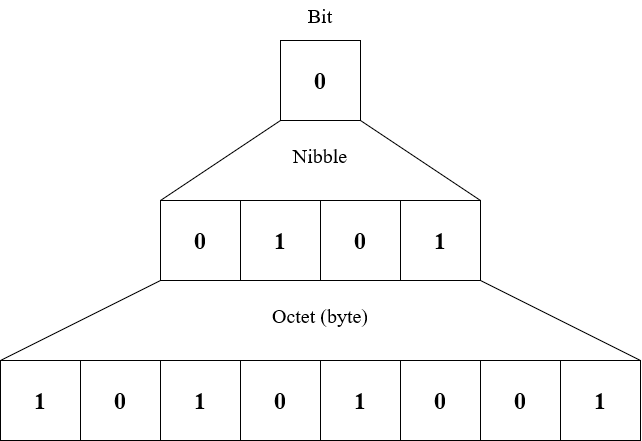
\includegraphics[width=0.5\textwidth]{byte.png}
 \end{figure}

Octet-ul va reprezenta unitatea fundamentală și indivizibilă pentru microarhitectura microprocesorul dezvoltat prin această lucrare. Acesta, prin urmare, este cea mai mică entitate adresabilă cu care se va lucra. Un octet este limitat de numărul de date pe care le poate reprezenta, acestea fiind calculate prin exponentul $\ 2^n$, în cazul nostru, $\ 2^8$ sau 256 de valori.

Un lucru important de menționat este că valoarea maximă a unui număr pe \textit{n} biți va fi mereu $\ 2^n -1$. Prin urmare, dacă dorim să reprezentăm o putere oarecare $\ 2^n$, vor fi necesari $\ n +1$ biți de date.
Tabelul \ref{Tabela:2} prezintă realația dintre magnitudinea binară (număul de biți folosiți în reprezentare) și cantitata de date reprezentate prin plaja de valori adiacentă, ignorând existenta numerelor negative.

\begin{table}[h]
\centering
\caption{Plaja de valori asumând numere strict pozitive, de magnitudini binare diverse }
\label{Tabela:2}
\begin{tabular}{ ||c|c|c|| }
 \hline
 Biți de date & Numărul datelor & Interval valori \\ 
 \hline  \hline
 8 & 256 & $\ 0 \le n \le 2^{8} - 1$ \\
 \hline
 16 & 65536 & $\ 0 \le n \le 2^{16} - 1$ \\
 \hline
 32 &  $\ 2^{32}$ & $\ 0 \le n \le 2^{32} - 1$ \\
 \hline
 64 & $\ 2^{64}$ & $\ 0 \le n \le 2^{64} -1$ \\
 \hline
\end{tabular}
\end{table}

\subsubsection{BAZA HEXADECIMALĂ}
Datorită clarificării reprezentării datelor în radix-ul binar, întelegerea bazei hexadecimale va fi cu atât mai simplă. Convertirea unui număr din binar in hexadecimal se face pe baza împărțirii acestuia în serii de \textit{nibble}. În situația când reprezentarea binară nu are destui biți pentru a acomoda o așa diviziune a sa, se completează cu diferența de simboluri de 0 necesare. Tabela \ref{Tabela:3} prezintă valorile care vor fi utilizate în conversie cât și echivalența dintre baza binară, decimală și hexadecimală.

\begin{table}[h]
\centering
\caption{Echivalența nibble - simbol hexadecimal }
\label{Tabela:3}
\begin{tabular}{ ||c|c|c|| }
 \hline
 Nibble & Simbol & Decimal\\ 
 \hline  \hline
 0000 & 0 & 0\\
 \hline
 0001 & 1 & 1\\
 \hline
 0010 & 2 & 2\\
 \hline
 0011 &  3 & 3\\
 \hline
 0100 & 4 & 4\\
 \hline
 0101 & 5 & 5 \\
 \hline
 0110 & 6 & 6\\
 \hline
 0111 & 7 & 7\\
 \hline
 1000 & 8 & 8\\
 \hline
 1001 & 9 & 9\\
 \hline
 1010 & A & 10\\
 \hline
 1011 & B & 11\\
 \hline
 1100 & C & 12\\
 \hline
 1101 & D & 13\\
 \hline
 1110 & E & 14\\
 \hline
 1111 & F & 15\\
 \hline
\end{tabular}
\end{table}

\subsubsection{OPERAȚIILE MATEMATICE ȘI NUMERELE BINARE}
Pentru a utiliza în mod corect reprezentările în această bază, modul în care calculele matematice sunt efectuate asupra numerelor binare necesită clarificare.

Datele nu sunt folositoare doar prin existența lor. Pentru a dobândi utilitate, acestea sunt supuse aparatului matematic, prin care se calculează diverse valori, asumând un algoritm corect, care ne oferă informații despre problema pe care dorim să o rezolvăm.

Cea mai elementară operație matematică care poate fi aplicată unui număr este adunarea. Însumarea numerelor este cu atât mai facilă cu cât numărul de simboluri folosite în reprezentarea acestora scade. Spre norocul lumii digitale, radix-ul utilizat permite efectuarea operațiilor matematice în cele mai simple metode. Există doar $\ 4$ operații fundamentale posibile, acestea fiind prezentate în Tabela \ref{Tabela:3}.

\begin{table}[h]
\centering
\caption{Operațiile fundamentale de însumare a numerelor binare }
\label{Tabela:4}
\begin{tabular}{ ||c|c|c|| }
 \hline
 Operație & Sumă & Carry \\ 
 \hline  \hline
 0 + 0 & 0 & 0\\
 \hline
 0 + 1 & 1  & 0\\
 \hline
 1 + 0 &  1 & 0 \\
 \hline
 1 + 1 & 0 & 1 \\
 \hline
\end{tabular}
\end{table}
Dintre toate aceste operații, cea căreia îi vom oferi o importanță ridicată este $\ 1 + 1 = 0$ \textit{carry} 1. Aceasta  ne obligă să adunăm o unitate bițiilor de pe poziții superioare. Practic, acestă sumă, odată ce este generalizată, ne spune că $\ 2^n + 2^n = 2 \cdot 2^n = 2^{n+1}$, o trivialitate matematică. Diverse exemple de adunare ale numerelor binare pot fi consultate în Figura \ref{Figura:2}.

 \begin{figure}[h!]
 \centering
 \caption{Exemple de adunare a numerelor binare}
 \label{Figura:2}
 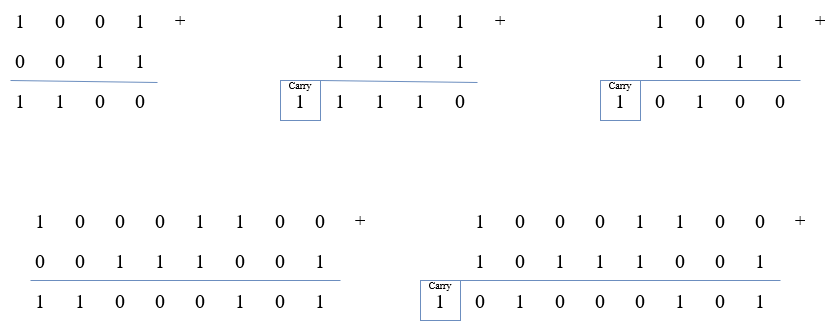
\includegraphics[width=0.9\textwidth]{binary_addition.png}
 \end{figure}

\subsubsection{REPREZENTAREA NUMERELOR NEGATIVE}
Modul în care numerele positive sunt adunate fiind acum clarificat, următoara operație matematică tratată este scăderea. Aceasta poate fi vizualizată ca adunarea unui numar \textit{a} la inversul aditiv al altui număr \textit{b}.
Această operație cere prin urmare un mod de reprezentare al numerelor binare negative, soluție care vine prin trei metode.

Primul mod de reprezentare este cel prin semn-magnitudine. Acesta este intuitiv, fiind similar cu reprezentarea numerelor decimale cu semn. Bit-ul cel mai semnificativ devine acum bit-ul de semn, 1 reprezentând un număr negativă, iar 0 unul pozitiv. Tabelul \ref{Tabela:4} prezintă aplicarea acestei reprezentări asupra numerelor pe 8 biți.

\begin{table}[h]
\centering
\caption{Reprezentarea prin semn-magnitudine }
\label{Tabela:5}
\begin{tabular}{ ||c|c|c|| }
 \hline
 Valoare binară & Semn magnitudine &  Fără semn\\ 
 \hline  \hline
 00000000 & 0 & 0\\
 \hline
 00000001 & 1  & 1\\
 \hline
 00000010 &  2 & 2 \\
 \hline
  ... &  ... & ... \\
 \hline
 01111110 & 126 & 126 \\
 \hline
 01111111 & 127 & 127 \\
 \hline
 10000000 & -0 & 128 \\
 \hline
 10000001 & -1 & 129 \\
 \hline
 10000010 & -2 & 130 \\
 \hline
   ... &  ... & ... \\
 \hline
  11111101 & -125 & 253 \\
 \hline
 11111110 & -126 & 254 \\
 \hline
 11111111 & -127 & 255 \\
 \hline
\end{tabular}
\end{table}
Se pot astfel distinge următoarele lucruri:
\begin{itemize}
\item Există două reprezentări posibile pentru 0, și anume $\ \pm 0$.
\item Deși se acopera tot 255 de valori numerice posibile (256 cu cel de al doilea 0), plaja de valori \textit{signed} s-a distribuit egal numerelor negative și celor pozitive. Astfel, numerele \textit{unsigned} semn-magnitudine  sunt cuprinse în intervalul $\ [-2^{n-1}+1, 2^{n-1}-1]$ unde $\ n > 0$ 
\end{itemize}

O altă medotă de reprezentare este prin complementul de 1. Conform acesteia, se inversează biții numărului binar pozitiv (biții cu valoarea 1 vor deveni 0 și viceversa) rezultând astfel inversul său aditiv. Spre exemplu, $\ 00000001' = 11111110;$ $\ 01010101' = 10101010$ iar, în cazul lui 0, $\ 00000000' = 11111111$. Tabela \ref{Tabela:5} conține reprezentările numerelor de 8 biți.
\begin{table}[h]
\centering
\caption{Reprezentarea prin complement de 1 }
\label{Tabela:6}
\begin{tabular}{ ||c|c|c|| }
 \hline
 Valoare binară & Semn magnitudine &  Fără semn\\ 
 \hline  \hline
 00000000 & 0 & 0\\
 \hline
 00000001 & 1  & 1\\
 \hline
 00000010 &  2 & 2 \\
 \hline
  ... &  ... & ... \\
 \hline
 01111110 & 126 & 126 \\
 \hline
 01111111 & 127 & 127 \\
 \hline
 10000000 & -127 & 128 \\
 \hline
 10000001 & -126 & 129 \\
 \hline
 10000010 & -125 & 130 \\
 \hline
   ... &  ... & ... \\
 \hline
  11111101 & -2 & 253 \\
 \hline
 11111110 & -1 & 254 \\
 \hline
 11111111 & -0 & 255 \\
 \hline
\end{tabular}
\end{table}

La fel ca în cazul reprezentării prin semn-magnitudine, 0 dorește să respecte principiul superpoziției, diferența pricipală însă, precum se distinge din compararea Tabelei \ref{Tabela:5} cu  Tabela \ref{Tabela:4}, este faptul ca valorile negative sunt eșalonate invers.

Problema acestor reprezentări este cu atât mai vizibilă când se efectuează adunarea a două numere binare, rezultatul fiind mereu $\ 111..1..111$, unda dintre reprezentările posibile ale lui 0. Soluția vine prin complementul de 2, complement format prin adăugarea unei unități reprezentării complementare de 1. Efectul însumării unitare este cel mai bine explicitat de Figura \ref{Figura:3}.
 
 \begin{figure}[h!]
 \centering
 \caption{Efectul adunării unității asupra complementului de 1}
 \label{Figura:3}
% https://q.uiver.app/#q=WzAsMjYsWzQsMCwiMDAwMDAwMDAgPSAxMTExMTExMSJdLFs0LDEsIjAiXSxbNCw0LCIwIl0sWzQsMywiMDAwMDAwMDAiXSxbMiw0LCIuLi4iXSxbMiwxLCIuLi4iXSxbNiwxLCIuLi4iXSxbNiw0LCIuLi4iXSxbMCw0LCItMTI4Il0sWzMsNCwiLTEiXSxbNSw0LCIxIl0sWzUsMywiMDAwMDAwMDEiXSxbNyw0LCIxMjciXSxbNywzLCIwMTExMTExMSJdLFs1LDEsIjEiXSxbNSwwLCIwMDAwMDAwMSJdLFs3LDEsIjEyNyJdLFs3LDAsIjAxMTExMTExIl0sWzMsMSwiLTEiXSxbMywwLCIxMTExMTExMCJdLFszLDMsIjExMTExMTExIl0sWzEsMSwiLTEyNyJdLFsxLDQsIi0xMjciXSxbMSwwLCIxMDAwMDAwMCJdLFsxLDMsIjEwMDAwMDAwIl0sWzAsMywiMTAwMDAwMDAiXSxbMiw5XSxbMiwxMF0sWzEwLDddLFs3LDEyXSxbMSwxNF0sWzE0LDZdLFs2LDE2XSxbMSwxOF0sWzE4LDIwLCIrMSIsMV0sWzIwLDldLFsxOCw1XSxbOSw0XSxbNSwyMV0sWzQsMjJdLFsyMiw4XSxbMjEsMjQsIisxIiwxXSxbMjQsMjJdXQ==
\[\begin{tikzcd}[cramped,column sep=tiny,row sep=scriptsize]
	& 10000000 && 11111110 & {00000000 = 11111111} & 00000001 && 01111111 \\
	& {-127} & {...} & {-1} & 0 & 1 & {...} & 127 \\
	\\
	10000000 & 10000000 && 11111111 & 00000000 & 00000001 && 01111111 \\
	{-128} & {-127} & {...} & {-1} & 0 & 1 & {...} & 127
	\arrow["{+1}"{description}, from=2-2, to=4-2]
	\arrow[from=2-3, to=2-2]
	\arrow[from=2-4, to=2-3]
	\arrow["{+1}"{description}, from=2-4, to=4-4]
	\arrow[from=2-5, to=2-4]
	\arrow[from=2-5, to=2-6]
	\arrow[from=2-6, to=2-7]
	\arrow[from=2-7, to=2-8]
	\arrow[from=4-2, to=5-2]
	\arrow[from=4-4, to=5-4]
	\arrow[from=5-2, to=5-1]
	\arrow[from=5-3, to=5-2]
	\arrow[from=5-4, to=5-3]
	\arrow[from=5-5, to=5-4]
	\arrow[from=5-5, to=5-6]
	\arrow[from=5-6, to=5-7]
	\arrow[from=5-7, to=5-8]
\end{tikzcd}\]
\end{figure}
Din această figură se observa următoarele:
\begin{itemize}
\item În cazul complementului de 2, nu mai există două reprezentări posibile pentru 0, locul suplimentar fiind luat de posibilitatea reprezentării unui număr negativ adițional, $\ -128$.
\item Intervalul posibil de valori devine acum  $\ [-2^{n-1}, 2^{n-1}-1]$.
\end{itemize}

Odată cu clarificarea reprezentării numerelor binare negative, operațiile matematice fundamentale pe care microprocesorul modelat pe decursul acestei lucrări le va utiliza, pot fi acum implementate. Însă, pentru a face legătura dintre abstractul arhitectural al sistemului și datele numerice, este necesară tratarea entităților digitale fundamentale cunoscute drept porți logice. 
\end{document}